% File: main.tex
% Custom LaTeX template for research papers
% Make sure you have 'custom.sty' and 'custom.bst' files in the same directory

\documentclass[letterpaper]{article}
\usepackage{custom}
\usepackage{times}
\usepackage{helvet}
\usepackage{courier}
\usepackage[hyphens]{url}
\usepackage{graphicx}
\urlstyle{rm}
\def\UrlFont{\rm}
\usepackage{natbib}
\usepackage{caption}
\frenchspacing
\setlength{\pdfpagewidth}{8.5in}
\setlength{\pdfpageheight}{11in}

% Recommended packages
\usepackage{booktabs}
\usepackage{subcaption}
\usepackage{amsmath}
\usepackage{amssymb}
\usepackage{multirow}
\usepackage{xcolor}
\usepackage{siunitx}
\usepackage{microtype}

% Improved formatting controls
\clubpenalty=10000  % Prevent orphans (single line at bottom of page)
\widowpenalty=10000 % Prevent widows (single line at top of page)
\displaywidowpenalty=10000
\predisplaypenalty=10000 % Avoid breaks before equations

% Declare custom units
\DeclareSIUnit\mebibyte{MiB}
\DeclareSIUnit\gram{g}
\DeclareSIUnit\watt{W}
\DeclareSIUnit\hour{h}
\DeclareSIUnit\second{s}

% PDF Info
\pdfinfo{
/TemplateVersion (2025.1)
}

% Section numbering depth
\setcounter{secnumdepth}{2}

% TITLE & AUTHOR
\title{Energy-Efficient Deep Learning Without Backpropagation: A~Rigorous Evaluation of Forward-Only Algorithms}

\author{
    Przemysław Spyra, Witold Dzwinel
}
\affiliations{
    AGH University of Krakow, Faculty of Computer Science \\
    \texttt{\{przspyra, dzwinel\}@agh.edu.pl}
}

\begin{document}

\maketitle

\begin{abstract}
The long-held assumption that backpropagation (BP) is essential for state-of-the-art performance is challenged by this work. We present rigorous, hardware-validated evidence that the Mono-Forward (MF) algorithm, a~backpropagation-free method, consistently surpasses an optimally tuned BP baseline in classification accuracy on its native Multi-Layer Perceptron (MLP) architectures. This superior generalization is achieved with profound efficiency gains, including up to \textbf{41\%} less energy consumption and up to \textbf{34\%} faster training. Our analysis, which charts an evolutionary path from Geoffrey Hinton's Forward-Forward (FF) to the Cascaded Forward (CaFo) and finally to MF, is grounded in a~fair comparative framework using identical architectures and universal hyperparameter optimization. We further provide a~critical re-evaluation of memory efficiency in BP-free methods, empirically demonstrating that practical overhead can offset theoretical gains. Ultimately, this work establishes MF as a~practical, high-performance, and sustainable alternative to BP for MLPs.
\end{abstract}

\section{Introduction}

Deep neural networks (DNNs) have achieved transformative success across AI \cite{krizhevsky2012imagenet, he2016deep, devlin2018bert}, yet this progress is built upon an escalating and unsustainable energy budget. As models scale, their operational requirements are projected to consume between 3\% and 4\% of global electricity by 2030 \cite{wef2025paradox}, with the training of a~single large model yielding a~carbon footprint equivalent to that of several automobiles \cite{abbas2024impact}.

The predominant training algorithm, backpropagation (BP), is the primary driver of this inefficiency \cite{rumelhart1986learning}. BP's dependence on a~full backward pass to compute gradients necessitates storing all intermediate activations, leading to high memory costs. Furthermore, its sequential nature imposes a~``backward locking'' bottleneck, which fundamentally constrains parallelization and prolongs training \cite{jaderberg2017decoupled}.

This sustainability crisis has spurred a~search for alternative algorithms free of backpropagation (BP free), inspired by the local and efficient learning principles of biological neural systems. This paper investigates an evolutionary progression of these methods:
\begin{itemize}
    \item \textbf{Forward-Forward (FF)} \cite{hinton2022forward}, a~foundational proof of concept demonstrating the viability of local, forward-only learning.
    \item \textbf{Cascaded Forward (CaFo)} \cite{zhao2023cafo}, a~structured evolution employing block-wise local classifiers to integrate supervisory signals more directly.
    \item \textbf{Mono-Forward (MF)} \cite{gong2025mono}, a~recent refinement using local projection matrices to achieve superior performance and efficiency.
\end{itemize}

While the potential of these algorithms is well recognized, a~comprehensive and fair evaluation based on direct hardware-level energy metrics remains insufficiently explored in the current literature. Existing work often overlooks architectural differences or inconsistent tuning practices, confounding the results \cite{desislavov2024energy}. This paper addresses this gap by conducting a~systematic, hardware-validated comparison of FF, CaFo, and MF against fairly tuned BP baselines on their respective native architectures.

\paragraph{Contributions}
The main contributions of this work are threefold:
\begin{itemize}
    \item \textbf{A~Rigorous Comparative Framework:} We establish a~transparent framework for the fair comparison of BP-free algorithms, mandating identical native architectures, universal hyperparameter tuning, and direct hardware-level efficiency measurements.
    \item \textbf{Validation of a~Superior BP-Free Algorithm:} We provide the first hardware-validated evidence that the Mono-Forward (MF) algorithm not only matches but surpasses backpropagation in both classification accuracy and training efficiency on MLP architectures.
    \item \textbf{An Empirical Re-evaluation of Memory Efficiency:} We conduct a~critical, empirical analysis of memory usage in BP-free methods, revealing that theoretical benefits are often counteracted by practical implementation overheads, thus correcting a~common misconception.
\end{itemize}

\section{An Evolution of BP Free Algorithms}

The high memory cost, sequential backward locking, and lack of biological plausibility of backpropagation have motivated a~search for alternative training paradigms \cite{lillicrap2020backpropagation, jaderberg2017decoupled}. This search has led to an evolution of BP free, forward only learning algorithms.

\paragraph{Forward-Forward (FF)}
Proposed by Geoffrey Hinton, the FF algorithm was a~foundational conceptual advance \cite{hinton2022forward}. It replaces the forward and backward passes of BP with two forward passes, one using ``positive'' (real) data and another using ``negative'' (contrastive) data. Each layer learns locally to distinguish between these data types by optimizing a~layer specific ``goodness'' metric. By eliminating the global backward pass, FF demonstrated that effective representation learning is possible with purely local objectives. However, its reliance on generating negative samples and its indirect goodness signal were identified as practical limitations, often leading to slow convergence and inefficient hardware utilization \cite{hinton2022forward, zhao2023cafo}.

\paragraph{Cascaded Forward (CaFo)}
The CaFo algorithm builds on FF by introducing a~more structured, block wise framework \cite{zhao2023cafo}. It comprises a~cascade of neural blocks, each followed by a~local predictor (an auxiliary classifier). This design provides a~more direct supervisory signal at multiple network depths, eliminating the need for negative samples. The neural blocks can be randomly initialized and fixed (`CaFo-Rand`) or trained with a~BP free method like Direct Feedback Alignment (`CaFo-DFA`). While CaFo addresses some of FF's limitations, it introduces a~critical trade-off, where `CaFo-Rand` suffers from poor feature quality on complex tasks, while `CaFo-DFA` improves accuracy but at a~significant computational cost for block pretraining \cite{zhao2023cafo}.

\paragraph{Mono-Forward (MF)}
MF represents a~recent refinement that simplifies and enhances the local learning mechanism \cite{gong2025mono}. Instead of using contrastive data or auxiliary classifiers, MF equips each hidden layer with a~dedicated, learnable projection matrix. This matrix directly maps the layer's activations to class specific ``goodness'' scores, upon which a~standard cross entropy loss is computed locally. Both the layer's primary weights and its projection matrix are updated using only this local loss signal. This elegant mechanism reportedly achieves accuracy that matches or surpasses BP on MLP architectures with significant efficiency gains, which motivated the rigorous validation in this work.

\section{Framework for Fair and Rigorous Comparison}

As a~key contribution of this work, we propose a~rigorous framework designed to isolate the impact of the training algorithm from confounding variables.

\paragraph{Fairness Protocols}
A~strict set of protocols was adhered to for all experiments:
\begin{enumerate}
    \item \textbf{Native Architecture Replication:} Each alternative algorithm was implemented on its native architecture as described in its source publication. FF and MF were evaluated on their designated MLP structures, while CaFo was evaluated on its defined three block CNN.
    \item \textbf{Identical Architectures for BP Baselines:} For each experiment, a~corresponding BP baseline was constructed using an \emph{identical} network architecture, omitting only algorithm specific components.
    \item \textbf{Systematic and Universal Hyperparameter Tuning:} Systematic hyperparameter optimization using the Optuna framework \cite{akiba2019optuna} was applied to \emph{all} algorithms, FF, CaFo, MF, and their respective BP baselines, for every configuration, maximizing validation set accuracy.
    \item \textbf{Consistent Early Stopping:} Training for all models was governed by a~consistent early stopping protocol based on validation performance. The model checkpoint yielding the best validation score was used for all final evaluations \cite{prechelt1998early}.
\end{enumerate}

\paragraph{Experimental Setup}
Experiments were conducted on the MNIST, Fashion-MNIST, CIFAR-10, and CIFAR-100 datasets. All experiments were executed on NVIDIA A100 40GB GPUs, with a~consistent software environment based on PyTorch v2.4.0 and CUDA 12.4.0. Full details are in Appendix B.

\paragraph{Evaluation Metrics}
A~comprehensive suite of metrics was employed:
\begin{itemize}
    \item \textbf{Performance:} Test set classification accuracy.
    \item \textbf{Efficiency (Direct Measurement):} Training Time (\si{\second}), Energy Consumption (\si{\watt\hour}, via NVML), and Peak Memory (\si{\mebibyte}, via NVML).
    \item \textbf{Efficiency (Estimation):} Forward pass GFLOPs (via PyTorch Profiler) and Estimated CO\textsubscript{2}e (\si{\gram}, via CodeCarbon).
\end{itemize}

\section{Experiments and Results}

The experiments chart a~clear evolutionary path from a~conceptually valid but impractical algorithm to a~highly effective and efficient solution.

\subsection{FF: A~Conceptually Sound Starting Point}

The experiments confirmed FF can achieve competitive accuracy on its native MLP architectures, validating its core premise. However, this comes at a~prohibitive efficiency cost (Table~\ref{tab:ff_bp_mlp_summary}), with its slow, volatile convergence causing up to a~\textbf{13x} longer training time and nearly \textbf{10x} greater energy use.

\begin{table}[htbp]
    \centering
    \caption{Performance and Efficiency: FF vs. BP on a~4x2000 MLP for Fashion-MNIST (Mean of 3 runs). Better results are bolded.}
    \label{tab:ff_bp_mlp_summary}
    \resizebox{\columnwidth}{!}{%
    \begin{tabular}{lcccc}
        \toprule
        Algorithm & Accuracy (\%) & Time (\si{\second}) & Energy (\si{\watt\hour}) & Peak Mem (\si{\mebibyte}) \\
        \midrule
        FF-AdamW & \textbf{89.63} & 574.60 & 14.28 & 1190 \\
        BP Baseline & 88.88 & \textbf{43.09} & \textbf{1.48} & \textbf{1168} \\
        \bottomrule
    \end{tabular}
    }
\end{table}

\begin{figure*}[t]
    \centering
    \begin{subfigure}[b]{0.48\textwidth}
        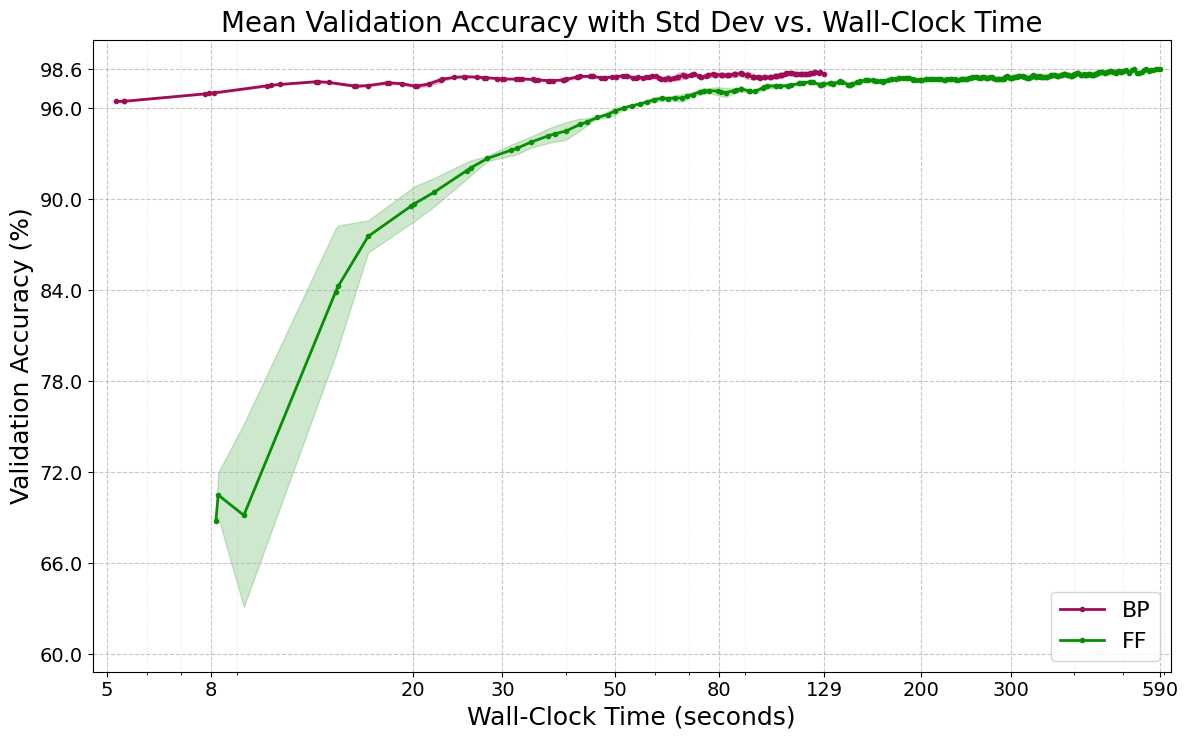
\includegraphics[width=\linewidth]{plots/FF_1.png}
        \caption{Validation Accuracy}
        \label{fig:ff_conv}
    \end{subfigure}
    \hfill
    \begin{subfigure}[b]{0.48\textwidth}
        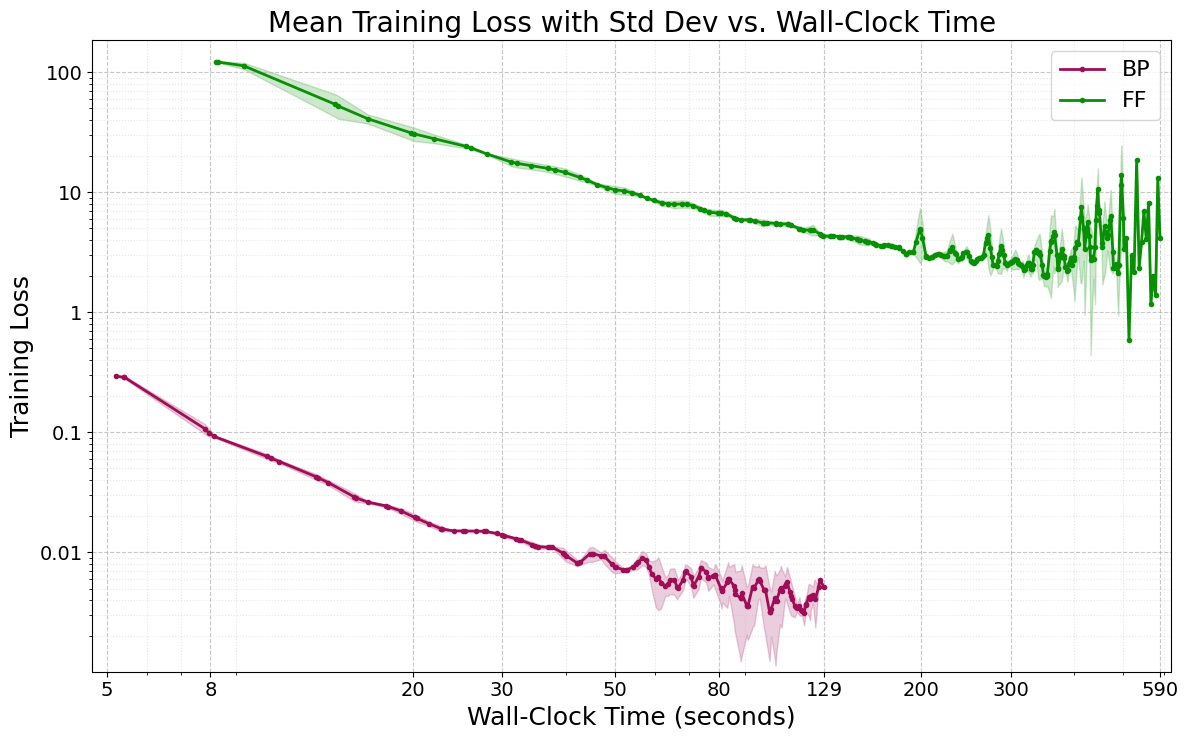
\includegraphics[width=\linewidth]{plots/FF_2.png}
        \caption{Training Loss}
        \label{fig:ff_loss}
    \end{subfigure}
    \caption{FF's slow convergence dynamics on the MNIST 4x2000 MLP, showing (a) significantly slower validation accuracy gains and (b) an erratic, high level training loss compared to BP's smooth optimization.}
    \label{fig:ff_convergence_dynamics}
\end{figure*}

The underlying cause is revealed by a~hardware level autopsy (Figure~\ref{fig:ff_resource_utilization}). The volatile GPU clock speeds for FF indicate inefficient hardware saturation compared to BP's stable, high utilization. Counterintuitively, FF also used slightly more peak memory than BP in the reported tests, refuting a~key presumed advantage. This inefficiency stems from FF's learning dynamics, as shown in Figure~\ref{fig:ff_convergence_dynamics}.

\begin{figure*}[t]
    \centering
    \begin{subfigure}[b]{0.48\textwidth}
        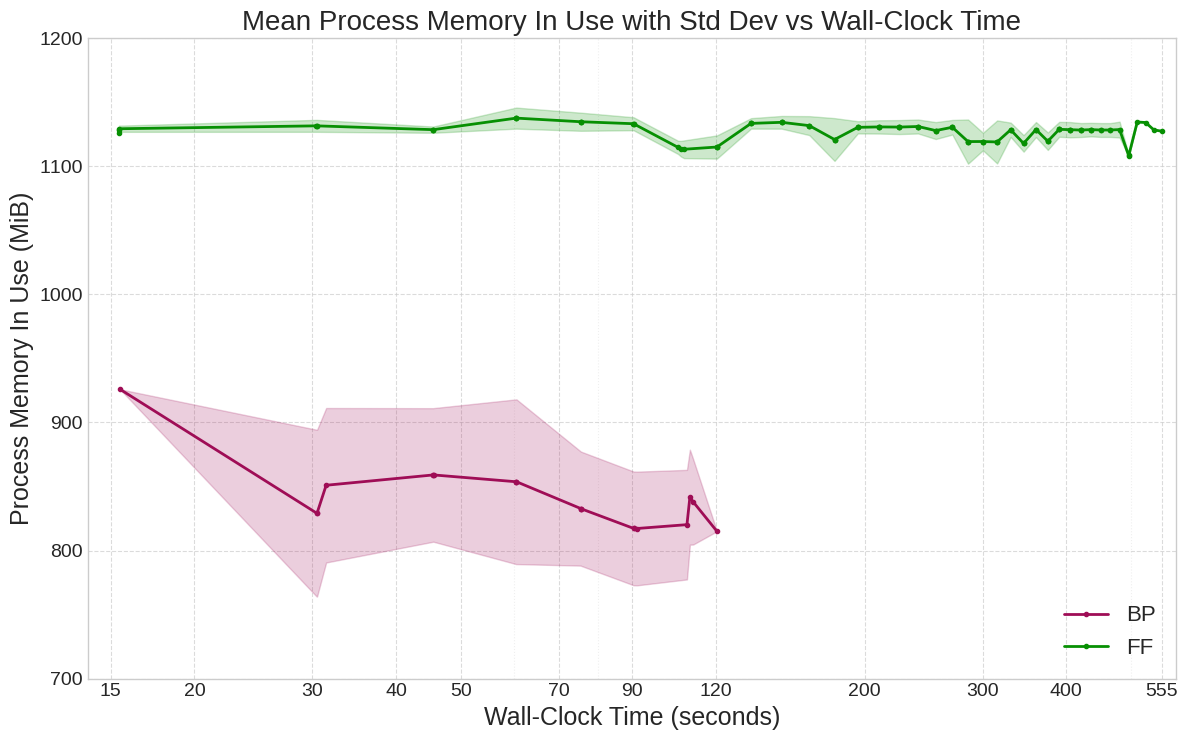
\includegraphics[width=\linewidth]{plots/FF_4.png}
        \caption{Memory Usage (\si{\mebibyte})}
        \label{fig:ff_mem}
    \end{subfigure}
    \hfill
    \begin{subfigure}[b]{0.48\textwidth}
        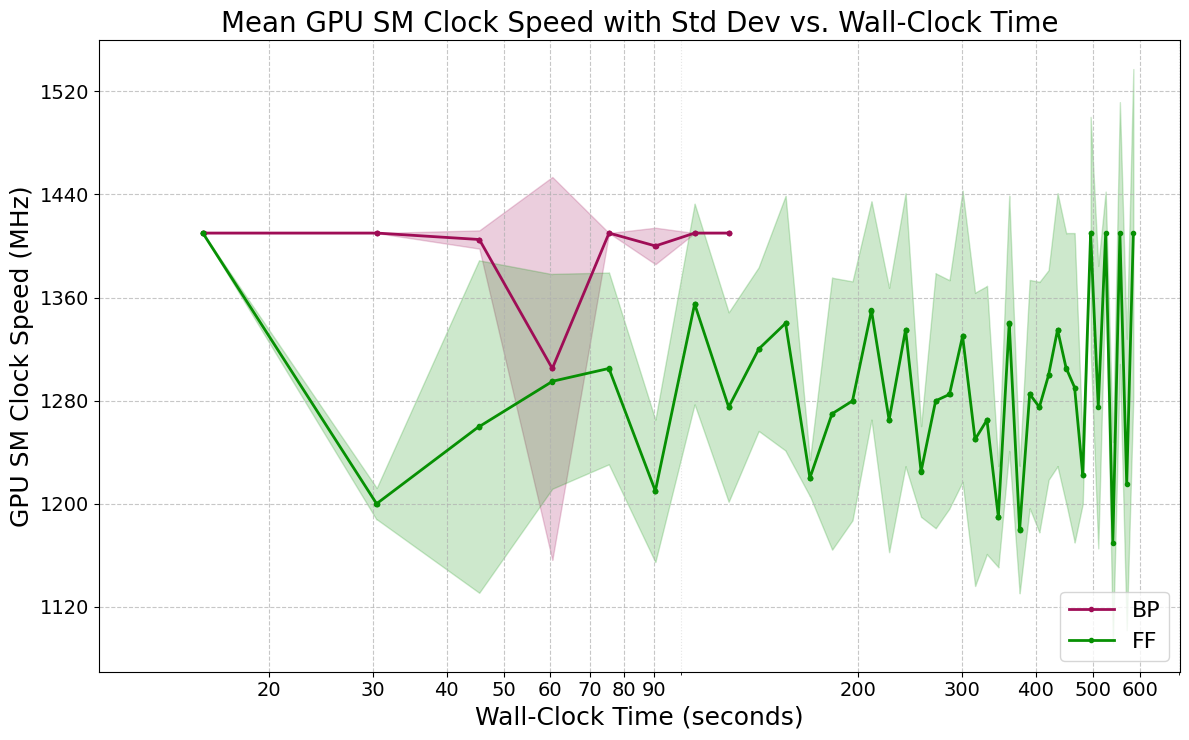
\includegraphics[width=\linewidth]{plots/FF_5.png}
        \caption{GPU Clock Speed (MHz)}
        \label{fig:ff_clock}
    \end{subfigure}
    \caption{The Hardware Autopsy of FF: (a) FF consumes slightly more peak memory than BP on this MLP. (b) Volatile GPU clock speeds reveal inefficient hardware utilization compared to BP's stable saturation.}
    \label{fig:ff_resource_utilization}
\end{figure*}

\subsection{CaFo: A~Structured Alternative with Acute Trade-offs}

The CaFo algorithm, evaluated on its native three block CNN, revealed a~stark trade-off contingent on its feature learning strategy. The `CaFo-Rand-CE` variant, using fixed random features, offered modest efficiency gains but at the cost of a~significant \textbf{13.23} percentage points drop in accuracy on CIFAR-10. Conversely, the `CaFo-DFA-CE` variant substantially improved accuracy but proved exceptionally resource intensive, consuming over \textbf{four times more} energy than BP on CIFAR-10. Figure~\ref{fig:cafo_convergence} illustrates these distinct learning dynamics, highlighting a~crucial insight that while high-quality features are essential for accuracy, the DFA mechanism used to learn them is computationally prohibitive.

\begin{figure*}[t]
    \centering
    \begin{subfigure}[b]{0.48\textwidth}
        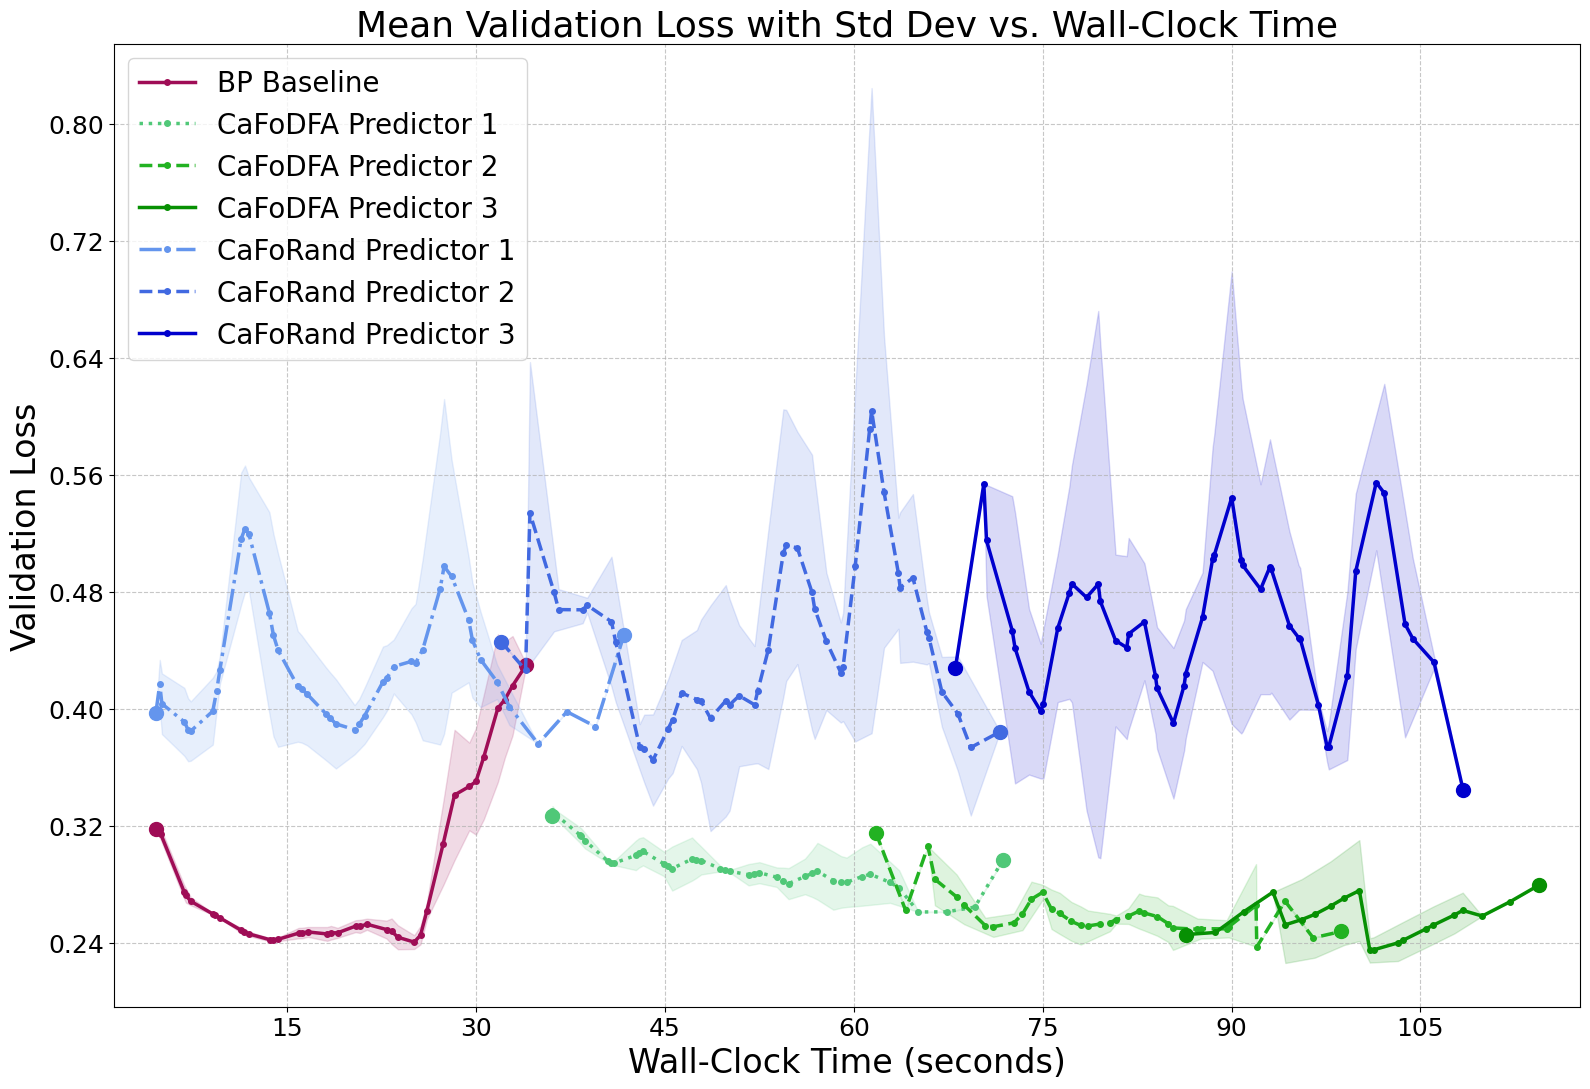
\includegraphics[width=\linewidth]{plots/Cafo_2.png}
        \caption{Validation Accuracy}
        \label{fig:cafo_acc}
    \end{subfigure}
    \hfill
    \begin{subfigure}[b]{0.48\textwidth}
        \includegraphics[width=\linewidth]{plots/Cafo_1.png}
        \caption{Validation Loss}
        \label{fig:cafo_loss}
    \end{subfigure}
    \caption{CaFo's Acute Trade-off on Fashion-MNIST: BP shows ideal convergence. CaFo-DFA is effective but incurs an upfront pretraining cost (flat line). CaFo-Rand is highly volatile, showing the necessity of quality features.}
    \label{fig:cafo_convergence}
\end{figure*}

\begin{figure*}[t]
    \centering
    \begin{subfigure}[b]{0.32\textwidth}
        \centering
        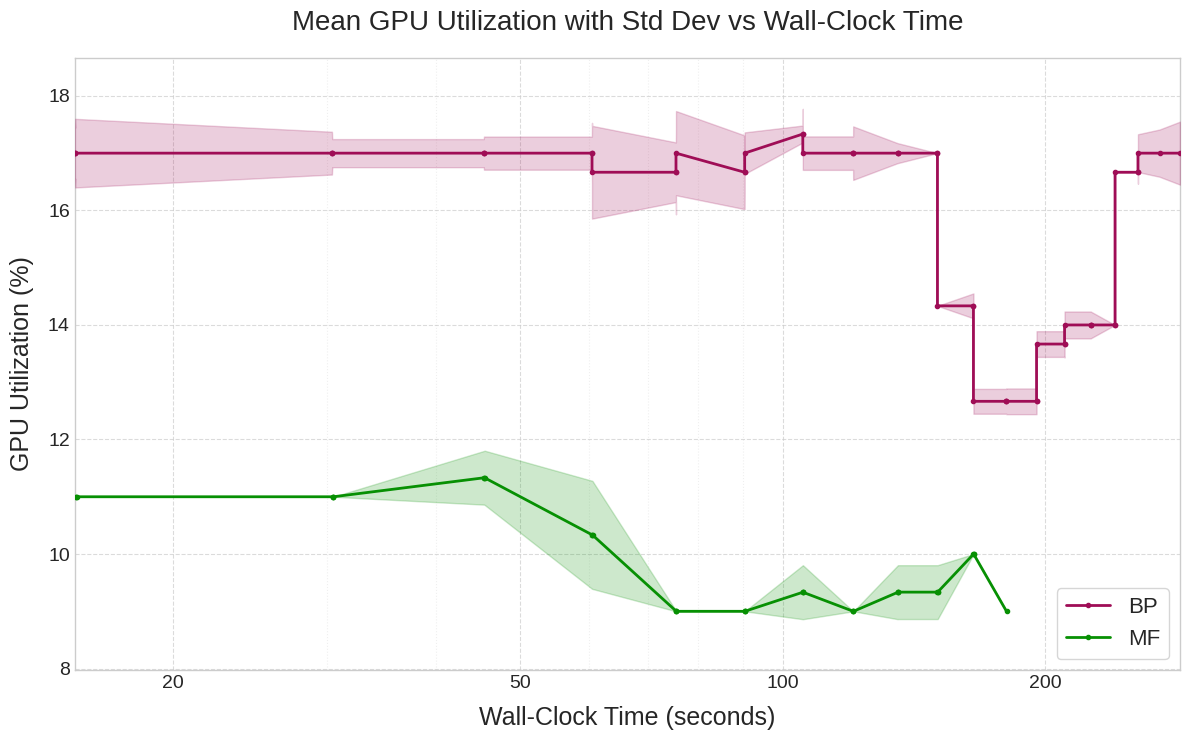
\includegraphics[width=\linewidth]{plots/mf_3.png}
        \caption{GPU Utilization (\%)}
        \label{fig:mf_utilization}
    \end{subfigure}
    \hfill
    \begin{subfigure}[b]{0.32\textwidth}
        \centering
        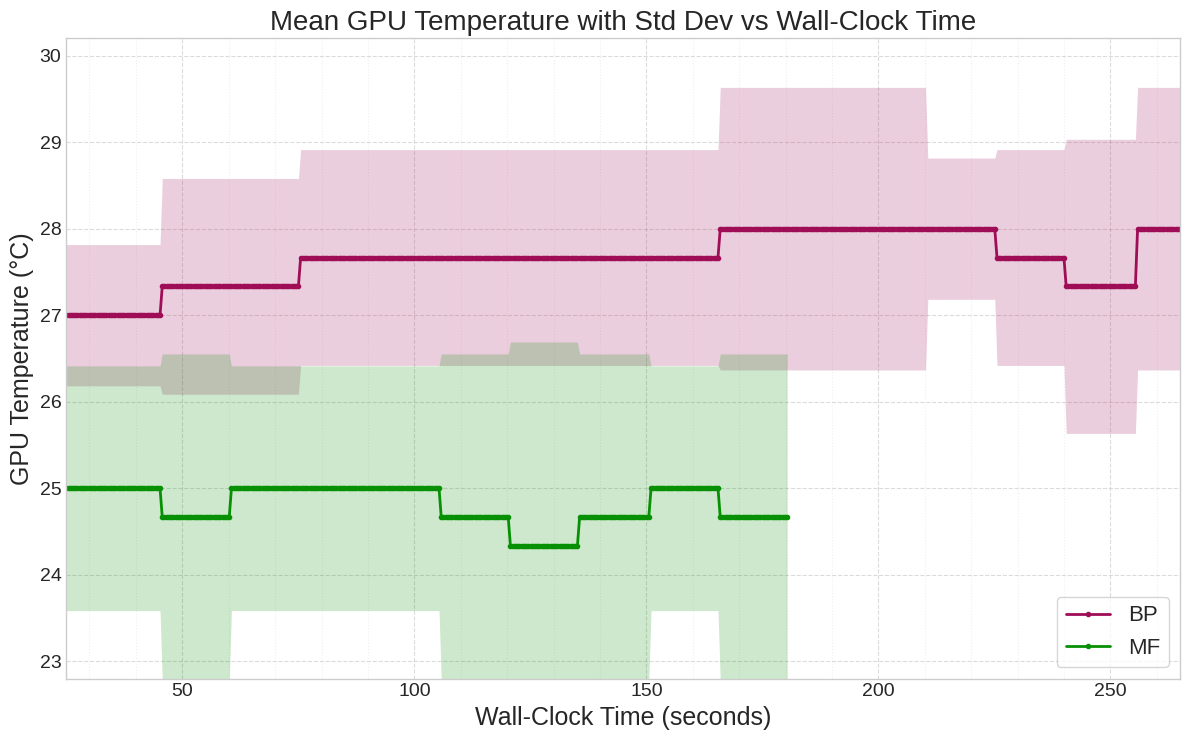
\includegraphics[width=\linewidth]{plots/mf_4.png}
        \caption{GPU Temperature (°C)}
        \label{fig:mf_temp}
    \end{subfigure}
    \hfill
    \begin{subfigure}[b]{0.32\textwidth}
        \centering
        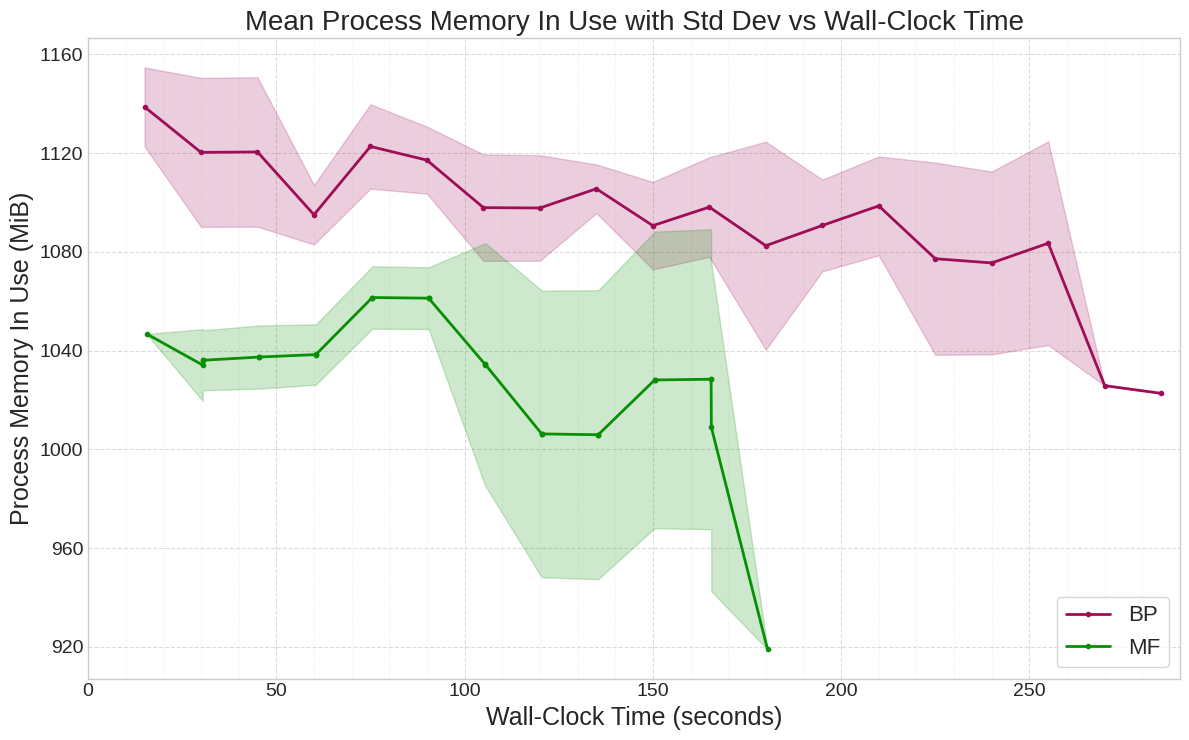
\includegraphics[width=\linewidth]{plots/MF_5.png}
        \caption{Process Memory In Use (\si{\mebibyte})}
        \label{fig:mf_memory_usage}
    \end{subfigure}
    
    \caption{Hardware monitoring plots for MF vs. BP on CIFAR-10. (a) MF's lower GPU utilization and (b) reduced thermal profile indicate superior energy efficiency. (c) The characteristic step like pattern in MF's memory usage serves as a~unique signature of its layer wise training mechanism.}
    \label{fig:mf_hardware_and_memory}
\end{figure*}

\subsection{MF: A~Breakthrough in Accuracy and Efficiency}

The Mono-Forward algorithm emerged as a~robust and high performing alternative, consistently matching or surpassing the classification accuracy of its fairly tuned BP baselines across all tested MLP architectures (Table~\ref{tab:mf_bp_perf_eff_summary}). This performance advantage was notable on every dataset, including a~significant \textbf{+0.51} percentage point gain on Fashion-MNIST and a~\textbf{+1.21} percentage point lead on the more complex CIFAR-10 task.

\begin{table}[htbp]
\centering
\caption{The MF Breakthrough: Performance \& Efficiency on CIFAR-10 3x2000 MLP Architecture (Mean of 3 runs). Best results are bolded.}
\label{tab:mf_bp_perf_eff_summary}
\resizebox{\columnwidth}{!}{%
\begin{tabular}{lcccc}
\toprule
Algorithm & Accuracy (\%) & Time (\si{\second}) & Energy (\si{\watt\hour}) & Peak Mem (\si{\mebibyte}) \\
\midrule
\textbf{MF} & \textbf{62.34} & \textbf{177.70} & \textbf{3.17} & \textbf{1120} \\
BP Baseline & 61.13 & 268.45 & 5.35 & 1184 \\
\bottomrule
\end{tabular}%
}
\end{table}

This superior accuracy was coupled with profound efficiency gains on the more demanding tasks. On the CIFAR-10 dataset, for instance, MF was \textbf{33.81\% faster} and consumed \textbf{40.78\% less energy} than BP. In contrast, the Fashion-MNIST result highlights a~different, compelling trade-off. Here, MF achieved superior accuracy by incurring a~minor increase in training time (+18\%) and energy (+10\%). This demonstrates the algorithm's ability to strategically trade a~small efficiency cost for a~meaningful performance gain. The key to its success lies in its learning dynamics. As shown in Figure~\ref{fig:mf_bp_cifar10_mlp_conv_curves}, MF's sequence of local optimizations converges to a~more favorable final validation loss compared to the global optimization of BP.

\begin{figure}[htbp]
\centering
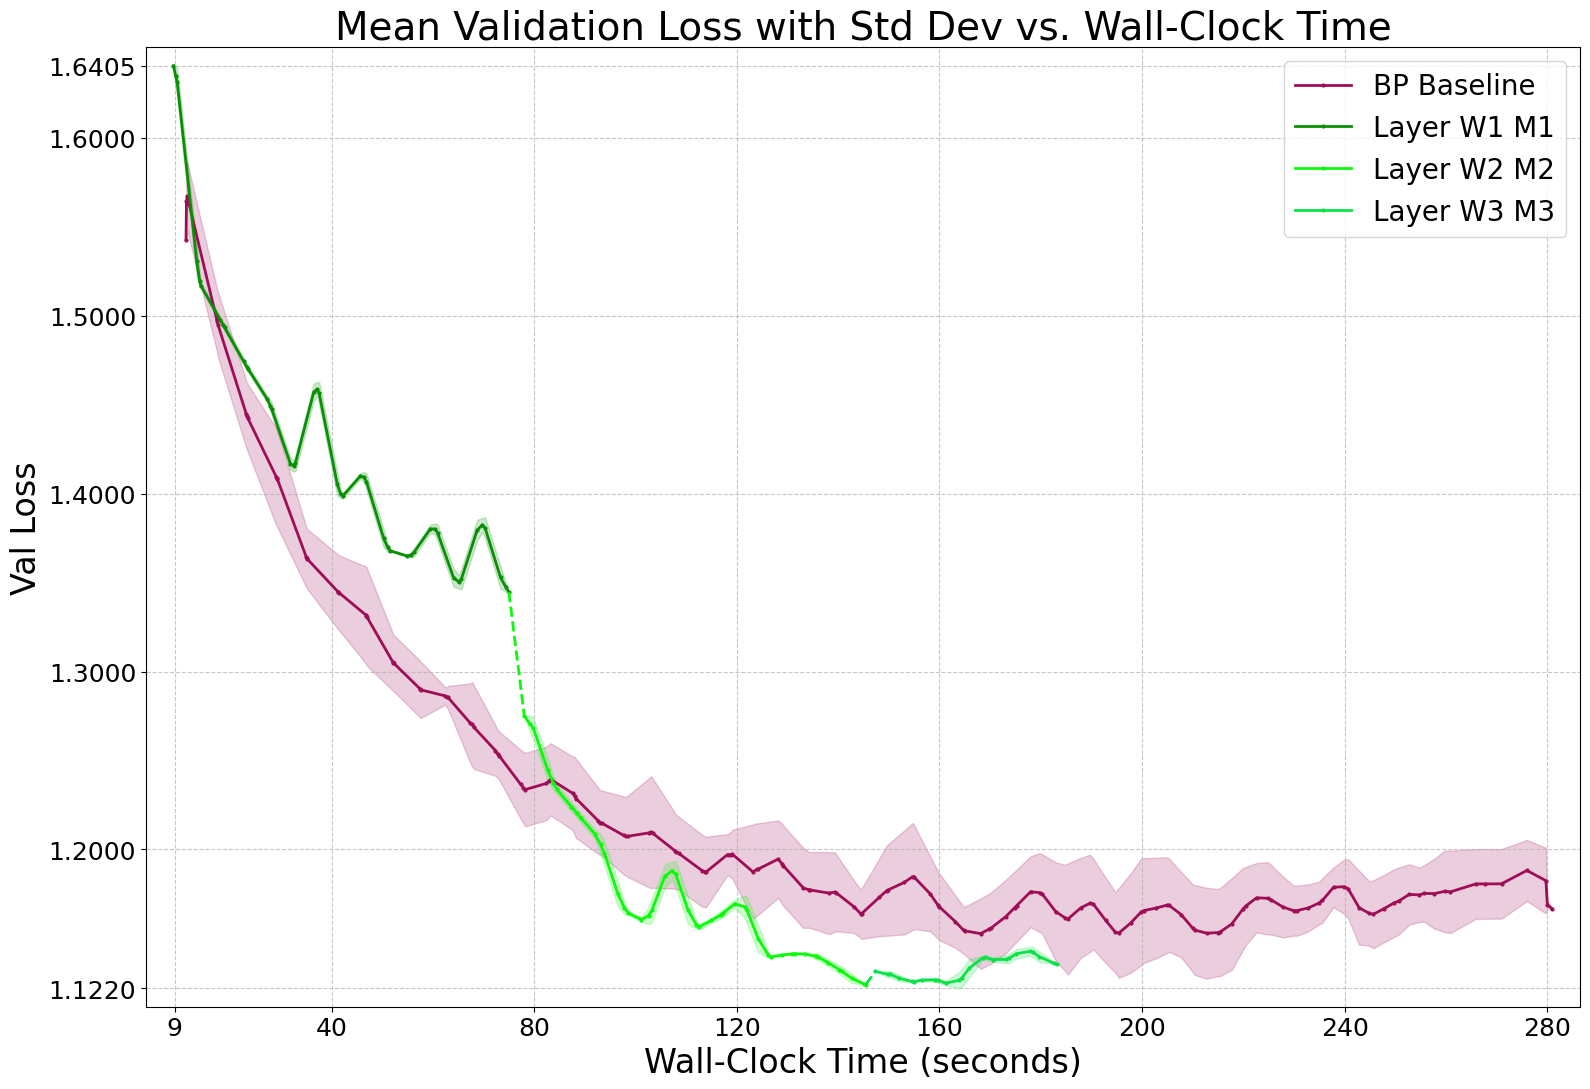
\includegraphics[width=0.9\columnwidth]{plots/mf_1.png} 
\caption{Explaining MF's Superior Generalization: MF's greedy local optimizations converge to a~more favorable (lower) final validation loss than BP's end-to-end global optimization on the CIFAR-10 3x2000 MLP, challenging the notion that global optimization is always superior.}
\label{fig:mf_bp_cifar10_mlp_conv_curves}
\end{figure}

Hardware monitoring further validates MF's lean design. As shown in Figure~\ref{fig:mf_hardware_and_memory}, its lighter computational load results in lower GPU utilization and a~reduced thermal profile. The algorithm's unique, layer wise training signature is also visible in its memory usage pattern.

A~complete summary comparing the relative performance and efficiency of each algorithm against its fair BP baseline across all tested configurations is presented in Appendix A (Tables~\ref{tab:appendix_ff_comparison}--\ref{tab:appendix_mf_comparison}).

\section{Discussion}

The empirical results demonstrate a~data-driven evolutionary progression among BP-free algorithms, culminating in the powerful and efficient Mono-Forward algorithm for MLPs. We analyze the underlying mechanisms, re-evaluate common assumptions, and explore the broader implications of these findings.

\subsection{Why MF Succeeds: The Power of Local Optimization}

FF's inefficiency stems from its slow convergence and suboptimal hardware utilization, while CaFo is constrained by a~trade-off requiring a~computationally prohibitive feature learning stage (DFA) for high accuracy.

MF succeeds by introducing local projection matrices, a~simple yet powerful mechanism. This allows each layer to compute a~direct, local classification loss, providing a~strong and efficient learning signal. The fact that MF converges to a~lower validation loss than end-to-end BP on identical MLPs (Figure~\ref{fig:mf_bp_cifar10_mlp_conv_curves}) is a~central finding. This suggests its greedy, layer-wise optimization acts as a~potent regularizer, guiding the model to a~parameter space with better generalization properties and challenging the paradigm that global optimization is a~prerequisite for state-of-the-art performance.

\subsection{Rethinking Memory Efficiency in BP-Free Learning}

A~critical insight is that eliminating the backward pass does not automatically guarantee superior memory efficiency. While CaFo-Rand showed modest memory savings, both FF and CaFo-DFA consumed \emph{more} memory than their BP baselines in our tests. Even MF's memory advantage on larger MLPs was modest at approximately 5\%.

This occurs because the practical overhead of the algorithms' unique components (e.g., FF's dual data streams, MF's projection matrices) can counteract the theoretical savings from not storing activations. This empirically grounded finding highlights the necessity of direct hardware measurement for a~complete resource analysis.

\subsection{Broader Implications: Toward Sustainable AI and Hardware Co-Design}

MF's substantial reduction in energy consumption offers a~concrete path toward more sustainable AI development, lowering the operational costs and carbon footprint of training MLP-based models. This efficiency also helps democratize AI by making high-performance training more accessible to researchers with limited computational resources.

Perhaps most profoundly, these results could influence future hardware design. The dominance of backpropagation has led to accelerators optimized for its forward-and-backward pass structure. The proven effectiveness of a~local algorithm like MF suggests that future accelerators could be designed differently. Chips optimized for local, forward-only computation might be simpler and more energy-efficient, as they would not require the complex data pathways and memory management for a~global backward pass. This work opens a~promising avenue for hardware-software co-design centered on BP-free principles.

\subsection{Limitations}

This work establishes MF's superiority on MLP architectures; however, its performance on other architectures like CNNs and Transformers remains an important open question. Future work should focus on adapting its projection matrix mechanism to these different paradigms to see if its compelling benefits can be generalized.

\section{Conclusion}

In this work, we conducted a~rigorous, fair, and hardware-validated comparison of three evolutionary stages of learning free of backpropagation. We demonstrated that while foundational algorithms like FF and CaFo present significant practical challenges, the recently proposed Mono-Forward (MF) algorithm represents a~breakthrough. On its native MLP architectures, MF consistently surpasses a~fairly tuned backpropagation baseline in classification accuracy across multiple benchmarks, while also delivering substantial efficiency gains, including up to a~\textbf{41\%} reduction in energy consumption on complex tasks. These findings challenge the paradigm that global optimization is essential for state-of-the-art performance and establish MF as a~practical, high-performance, and sustainable training algorithm for this class of networks. This research provides a~clear, data-driven path toward a~future of more efficient, accessible, and biologically plausible artificial intelligence.

\section*{Author Contributions}

The research was conducted as part of a~master's thesis by Przemysław Spyra, under the supervision of Witold Dzwinel. Przemysław Spyra was responsible for the development and implementation of the methodology, experiments, and analysis. Witold Dzwinel provided conceptual guidance, critical feedback, and helped shape the direction and presentation of the work.

\section*{Acknowledgments}

This work was supported by the Ministry of Science and Higher Education of Poland. The authors wish to thank the PLGrid Infrastructure for its support and ACK Cyfronet AGH for providing the computational resources on the Athena cluster, which were indispensable for this work. We gratefully acknowledge the AGH University of Science and Technology for providing the institutional support and academic environment that made this research possible.

\bibliography{bibliography}

\appendix
\section{Comprehensive Comparative Summary}
\label{app:full_comparison}

This appendix provides a~detailed summary of the relative performance and efficiency of each alternative algorithm compared to its corresponding fair backpropagation baseline across all experimental configurations. The metric $\Delta$Acc. is the absolute difference in percentage points; other $\Delta$ values are relative percentage differences. Positive accuracy and negative efficiency deltas favor the alternative algorithm.

\begin{center}
    \captionof{table}{Forward-Forward (FF) vs. BP Baseline on MLP Architectures.}\label{tab:appendix_ff_comparison}
    \resizebox{\columnwidth}{!}{%
    \begin{tabular}{l c c c c c}
        \toprule
        Dataset & Architecture & $\Delta$ Acc. (\%) & $\Delta$ Time (\%) & $\Delta$ Energy (\%) & $\Delta$ Mem. (\%) \\
        \midrule
        F-MNIST & MLP 4x2000 & +0.75 & +1233.26 & +862.35 & +1.88 \\
        MNIST & MLP 3x1000 & +0.24 & +342.11 & +339.95 & +0.85 \\
        MNIST & MLP 4x2000 & -0.01 & +305.08 & +236.88 & +1.88 \\
        \bottomrule
    \end{tabular}%
    }
\end{center}

\begin{center}
    \captionof{table}{Cascaded Forward (CaFo) vs. BP Baseline on 3-Block CNN Architecture.}\label{tab:appendix_cafo_comparison}
    \resizebox{\columnwidth}{!}{%
    \begin{tabular}{l c c c c c}
        \toprule
        Variant & Dataset & $\Delta$ Acc. (\%) & $\Delta$ Time (\%) & $\Delta$ Energy (\%) & $\Delta$ Mem. (\%) \\
        \midrule
        CaFo-Rand-CE & \multirow{2}{*}{MNIST} & -0.32 & +88.48 & +32.65 & -6.67 \\
        CaFo-DFA-CE & & +0.08 & +124.82 & +81.83 & +1.11 \\
        \cmidrule(lr){2-6}
        CaFo-Rand-CE & \multirow{2}{*}{F-MNIST} & +1.11 & +205.00 & +115.99 & -6.67 \\
        CaFo-DFA-CE & & +2.47 & +206.51 & +201.43 & +1.11 \\
        \cmidrule(lr){2-6}
        CaFo-Rand-CE & \multirow{2}{*}{CIFAR-10} & -13.23 & -2.96 & -19.24 & -8.98 \\
        CaFo-DFA-CE & & -1.72 & +287.17 & +301.94 & +1.26 \\
        \cmidrule(lr){2-6}
        CaFo-Rand-CE & \multirow{2}{*}{CIFAR-100} & -11.44 & +246.27 & +188.87 & -5.02 \\
        CaFo-DFA-CE & & -4.43 & +557.19 & +576.82 & +2.51 \\
        \bottomrule
    \end{tabular}%
    }
\end{center}

\begin{center}
    \captionof{table}{Mono-Forward (MF) vs. BP Baseline on MLP Architectures.}\label{tab:appendix_mf_comparison}
    \resizebox{\columnwidth}{!}{%
    \begin{tabular}{l c c c c c}
        \toprule
        Dataset & Architecture & $\Delta$ Acc. (\%) & $\Delta$ Time (\%) & $\Delta$ Energy (\%) & $\Delta$ Mem. (\%) \\
        \midrule
        MNIST & MLP 2x1000 & +0.09 & -12.07 & -13.34 & +0.86 \\
        F-MNIST & MLP 2x1000 & +0.51 & +18.20 & +9.90 & +0.86 \\
        \textbf{CIFAR-10} & \textbf{MLP 3x2000} & \textbf{+1.21} & \textbf{-33.81} & \textbf{-40.78} & \textbf{-5.41} \\
        CIFAR-100 & MLP 3x2000 & +0.37 & -1.28 & -12.48 & -4.19 \\
        \bottomrule
    \end{tabular}%
    }
\end{center}

\section{Computational Environment and Reproducibility}
\label{app:environment_appendix}

\subsection{Environment Details}
The experiments were conducted on the Athena cluster at ACK Cyfronet AGH.
\begin{itemize}
    \item \textbf{OS:} Rocky Linux 9.5
    \item \textbf{CPU:} AMD EPYC 7742 @ 2.25 GHz
    \item \textbf{GPU:} NVIDIA A100-SXM4-40GB
    \item \textbf{NVIDIA Driver:} 570.86.15
    \item \textbf{CUDA Toolkit:} 12.4.0
    \item \textbf{Framework:} PyTorch v2.4.0 (`+cu121`)
    \item \textbf{Python:} 3.10.4
    \item \textbf{Key Libraries:} numpy 2.2.4, scikit-learn 1.6.1, torchvision 0.19.0, optuna 4.2.1, pynvml 12.0.0, PyYAML 6.0.2, CodeCarbon 3.0.1, wandb 0.19.8
    \item \textbf{Energy and Resource Monitoring:} NVIDIA Management Library (NVML)
    \item \textbf{Carbon Estimation:} CodeCarbon v3.0.1 \cite{codecarbon2021}
\end{itemize}

\subsection{Code Repository}
To ensure full reproducibility, the complete source code, configuration files, and experimental logs have been made publicly available at:
\begin{center}
    \url{https://github.com/Przemyslaw11/BeyondBackpropagation}
\end{center}

\end{document}